\section{Styrkeberegning}
\subsection{Hjulbrakett}
Dette gjøres i UGS NX Nastran 7.5, Advanced Simulation. Kraften $F_{2}$ = 1720 N fordeles likt over de to hullene i hjulbraketten. Hjulbraketten settes som fast låst på undersiden.

\begin{figure}[H]
\begin{center}$
\begin{array}{ccc}
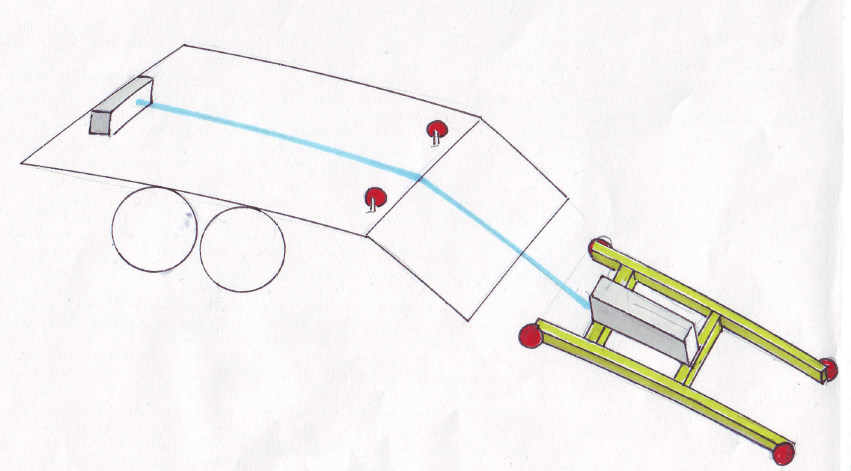
\includegraphics[width=2.5in]{images/Bilde_4.PNG} &
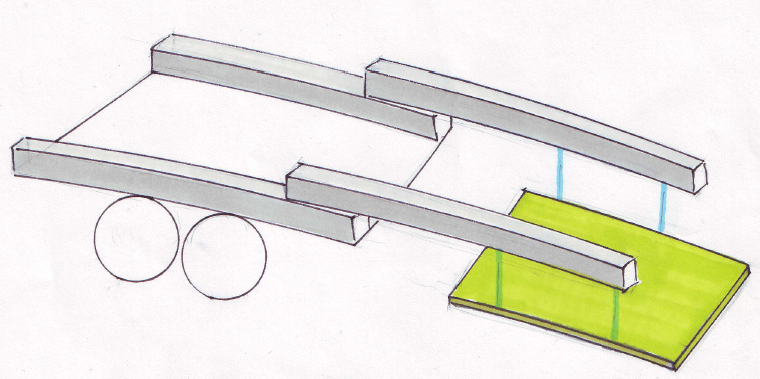
\includegraphics[width=2.5in]{images/Bilde_5.PNG} &  
\end{array}$
\end{center}
\caption{Krefter og grensebetingelser hjulbrakett}
\end{figure}

Simuleringen gir største spenning $\sigma_{max}$=105 MPa. Ser at denne vil oppstå i opplagerhullet til hjulets aksel, på den siden hvor skruehodet er forsenket.

\begin{figure}[H]
\begin{center}$
\begin{array}{ccc}
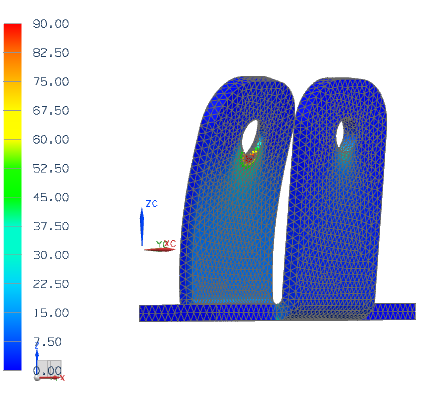
\includegraphics[width=2.0in]{images/Bilde_2.PNG} &
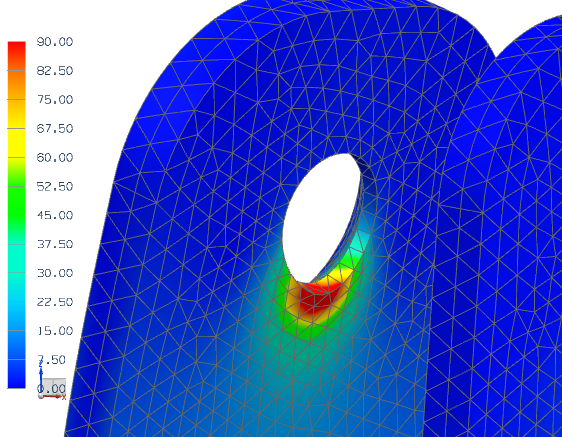
\includegraphics[width=2.0in]{images/Bilde_3.PNG} &  
\end{array}$
\end{center}
\caption{Von-Mises spenninger hjulbrakett}
\end{figure}

Ståltype S235JR som benyttes har flytgrense $\sigma_{ys}$=225 MPa. Kan ut ifra dette beregne sikkerheten mot at det oppstår flyt i materialet:

\begin{equation}
\eta=\frac{\sigma_{ys}}{\sigma_{max}}
\end{equation}

\begin{equation}
\eta=\frac{225 MPa}{105 MPa}=2.14
\end{equation}\\

Hjulbraketten vil ha en sikkerhet mot at det oppstår flyt i materialet på 2.14.

\subsection{Rammebrakett}

Setter på randbetingelser og krefter som vist nedenfor. Kraften $F_{1}$=1230 N fordeles likt over de to hullene på toppen. Rammebraketten settes som fast låst på undersiden.

\begin{figure}[H]
\begin{center}$
\begin{array}{ccc}
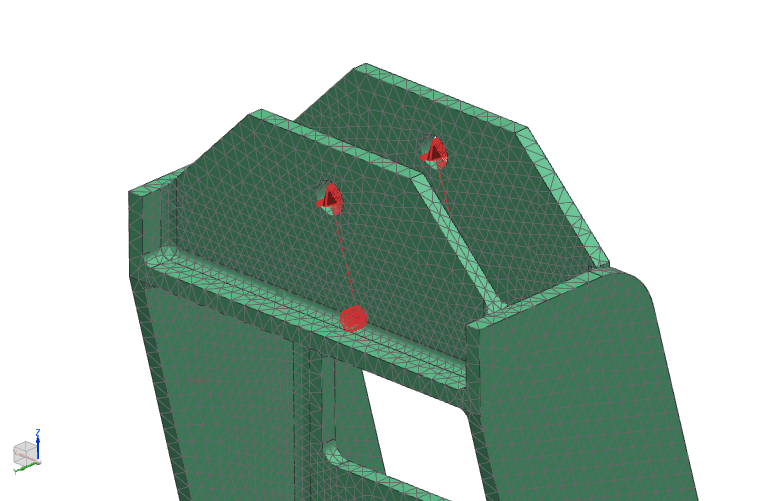
\includegraphics[width=2.5in]{images/Bilde_7.PNG} &
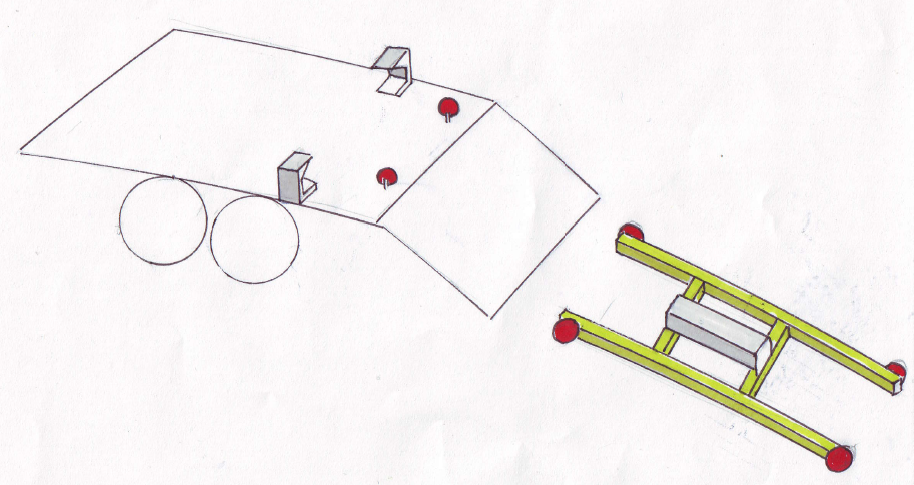
\includegraphics[width=2.5in]{images/Bilde_6.PNG} &  
\end{array}$
\end{center}
\caption{Krefter og grensebetingelser rammebrakett}
\end{figure}

Simuleringen gir største spenning $\sigma_{max}$=31 MPa. Denne oppstår inne i hullene hvor hjulet på toppen er opplagret.

\begin{figure}[H]
\begin{center}$
\begin{array}{ccc}
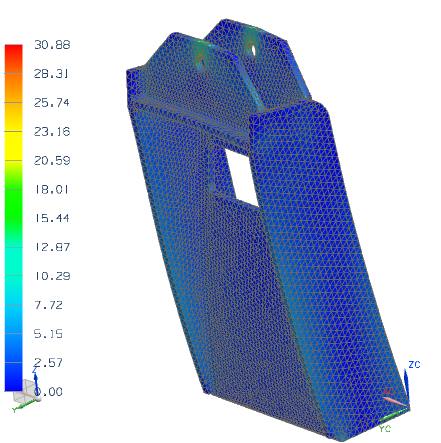
\includegraphics[width=2.0in]{images/Bilde_8.PNG} &
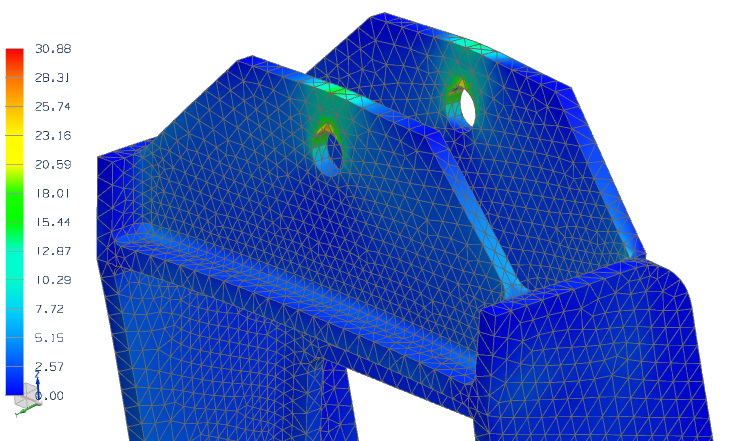
\includegraphics[width=3.0in]{images/Bilde_9.PNG} &  
\end{array}$
\end{center}
\caption{Von-Mises spenninger rammebrakett}
\end{figure}

Beregnet sikkerhet mot at det oppstår flyt i materialet:

\begin{equation}
\eta=\frac{225 MPa}{31 MPa}=7.25
\end{equation}\\

Modellen er modellert som en solid, der sveisene er simulert med chamfers og har a-mål 5 mm.\newline
Rammebraketten vil ha en sikkerhet mot at det oppstår flyt i materialet på 7.25.


\subsection{Bein og Beinbrakett}
Setter på randbetingelser og krefter som vist nedenfor. I beinbrakettens hull påføres det en kraft tilsvarende bilens og rammens vekt i dette opplageret, $F_{5}$=250N. Beinene må også sørge for å holde rammen stabil sideveis, samt framover og bakover. For å simulere dette påføres det krefter på $F_{6}$=$F_{7}$=100N nederst på beinet i x- og y-retning. Beinbraketten settes som fast låst på baksiden.

\begin{figure}[H]
\begin{center}$
\begin{array}{ccc}
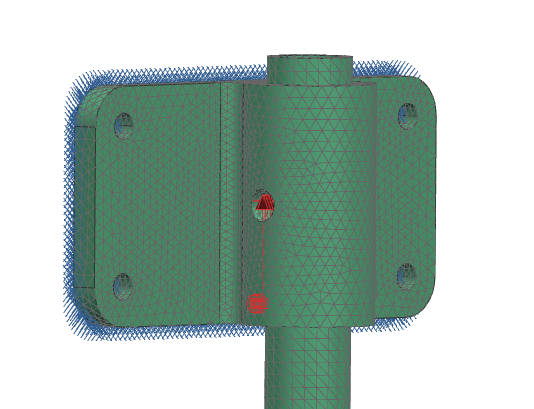
\includegraphics[width=2.5in]{images/Bilde_10.PNG} &
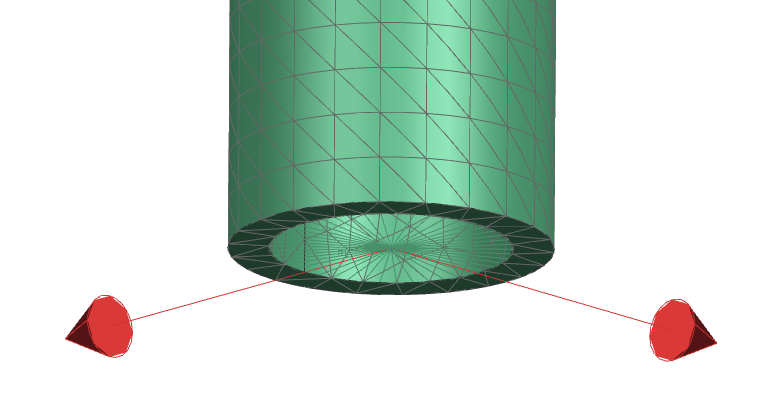
\includegraphics[width=2.5in]{images/Bilde_11.PNG} &  
\end{array}$
\end{center}
\caption{Krefter og grensebetingelser bein og beinbrakett}
\end{figure}

Simuleringen gir største spenning $\sigma_{max}$=85 MPa. Denne oppstår nederst på innfestingen mellom beinbraketten og beinet.

\begin{figure}[H]
\begin{center}$
\begin{array}{ccc}
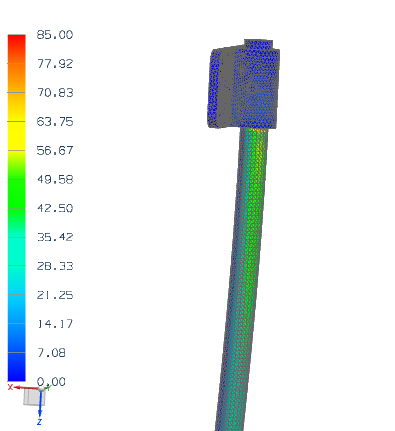
\includegraphics[width=2.0in]{images/Bilde_13.PNG} &
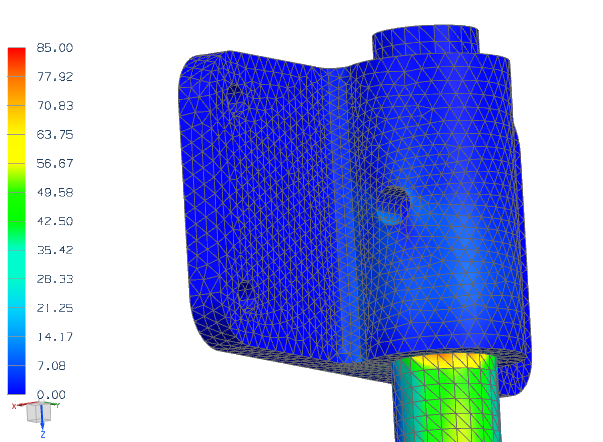
\includegraphics[width=3.0in]{images/Bilde_12.PNG} &  
\end{array}$
\end{center}
\caption{Von-Mises spenningerbein og beinbrakett}
\end{figure}

Beregnet sikkerhet mot at det oppstår flyt i materialet:

\begin{equation}
\eta=\frac{225 MPa}{85 MPa}=2.65
\end{equation}\\

Modellen er modellert som en solid, der sveisene er simulert med chamfers og har a-mål 20 mm.\newline
Beinet og beinbraketten vil ha en sikkerhet mot at det oppstår flyt i materialet på 2.65.
